\documentclass[a4paper]{article}

\usepackage[pages=all,color=black,position={current page.south},placement=bottom,scale=1,opacity=1,vshift=5mm]{background}
\SetBgContents{
    \ttfamily This work is shared under a \href{https://creativecommons.org/licenses/by-sa/4.0/}{CC BY-SA 4.0 license} unless otherwise noted
}

\usepackage[margin=1in]{geometry}
\usepackage{amsmath}
\usepackage{amssymb}
\usepackage[T2A]{fontenc}
\usepackage[utf8]{inputenc}
\usepackage[english,russian]{babel}
\usepackage{graphicx}
\usepackage{booktabs}
\usepackage{longtable}
\usepackage{array}
\usepackage{float}
\usepackage{hyperref}

\hypersetup{
    unicode,
    pdfauthor={},
    pdftitle={Влияние гауссовских и человекоподобных шумов на устойчивость моделей компьютерного зрения},
    pdfsubject={Исследование устойчивости сверточной сети к переносимым FGSM- и PGD-атакам},
    pdfkeywords={компьютерное зрение, состязательные атаки, гауссовский шум, человекоподобный шум, FGSM, PGD},
    pdfproducer={LaTeX},
    pdfcreator={pdflatex}
}

\title{Влияние гауссовских и человекоподобных шумов на устойчивость моделей компьютерного зрения}
\author{}
\date{}

\begin{document}

\maketitle

\begin{abstract}
В работе исследуется влияние гауссовских и человекоподобных шумов активаций и параметров на устойчивость сверточной нейронной сети к состязательным атакам. В гауссовской ветке сравнивались постоянный шум и его постепенное введение, а в человекоподобной ветке рассматривались латеральный, контрастно-адаптивный и пирамидальный шумы активаций, а также аксонный и дендритный шумы параметров. Модели оценивались на чистой выборке и на FGSM- и PGD-примерах, сформированных на исходной модели. Для человекоподобных шумов лучший результат составил 25{,}95\% для FGSM и 21{,}42\% для PGD. Однако независимо обученная модель без шума получила 28{,}64\% и 23{,}13\% соответственно. Следовательно, высокая точность на атакованных данных пока не может быть однозначно приписана шуму: значительная часть эффекта может объясняться неполной переносимостью атак между моделями с различной инициализацией.
\end{abstract}

\tableofcontents

\section{Введение}

Модели компьютерного зрения применяются в распознавании объектов, анализе медицинских изображений, автономных системах и других областях. При этом нейронные сети подвержены состязательным атакам: небольшие целенаправленные изменения входного изображения способны существенно изменить предсказание модели, хотя для человека изображение остается практически неизменным.

Одним из возможных способов повышения устойчивости является обучение модели в условиях внутренних возмущений. Такая модель не может опираться только на точные, но хрупкие признаки и должна формировать представления, устойчивые к вариациям сигнала и параметров. В данной работе проверяется гипотеза о том, что шумы, вдохновленные механизмами биологической зрительной системы, могут повысить устойчивость сверточной сети к атакам исходной модели.

Рассматриваемая оценка относится к переносимым атакам. FGSM- и PGD-примеры формируются на исходной модели, после чего без изменения используются для проверки всех остальных моделей. Поэтому полученные метрики не являются white-box оценкой исследуемых моделей.

\section{Архитектура модели}

Используется компактная сверточная сеть для классификации изображений CIFAR-10 размером $3\times32\times32$. Архитектура состоит из двух сверточных блоков и полносвязного классификатора. Модель содержит 1,117,162 обучаемых параметра.

\begin{figure}[H]
    \centering
    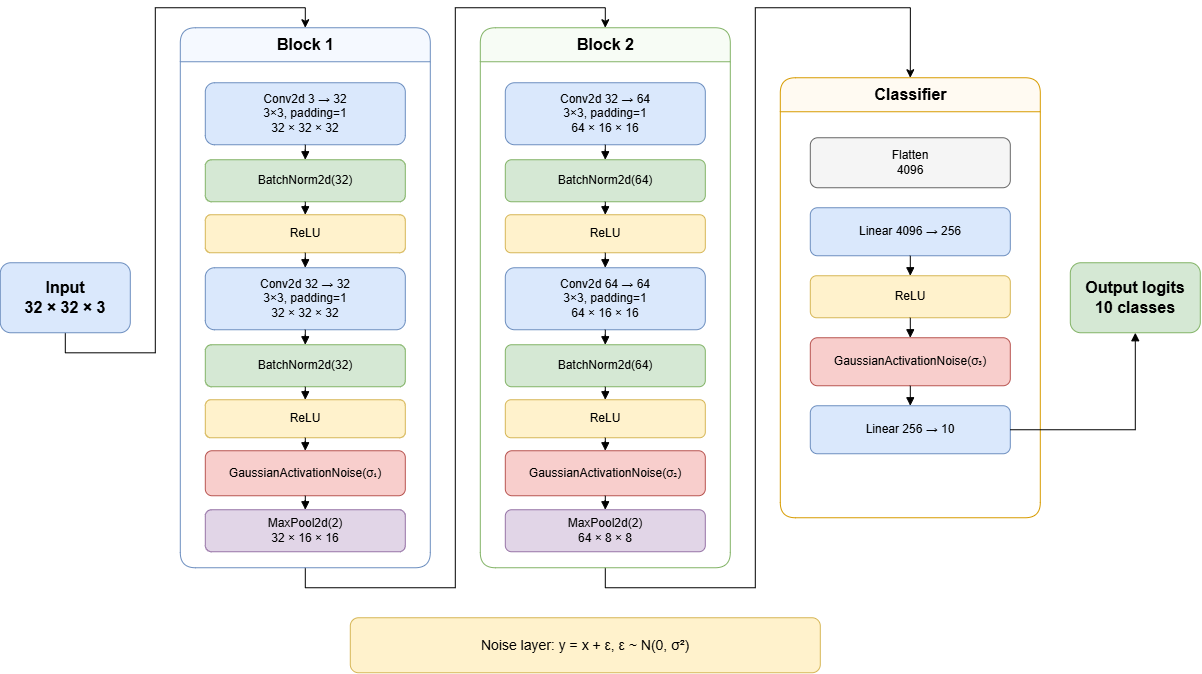
\includegraphics[width=0.88\linewidth]{src/net_architecture.png}
    \caption{Архитектура сверточной сети с блоками человекоподобных шумов}
    \label{fig:architecture}
\end{figure}

Первый блок содержит две свертки с 32 каналами и уменьшает пространственное разрешение до $16\times16$. Второй блок содержит две свертки с 64 каналами и формирует представление размера $64\times8\times8$. После выравнивания признаков используются полносвязные слои $4096\rightarrow256\rightarrow10$.

\section{Реализация человекоподобных шумов}

\subsection{Латеральное торможение}

После первой свертки первого блока генерируется белый шум, который фильтруется дискретным лапласианом

\begin{equation}
K=
\begin{pmatrix}
0 & -1 & 0\\
-1 & 4 & -1\\
0 & -1 & 0
\end{pmatrix}.
\end{equation}

Полученное пространственно коррелированное возмущение нормируется по стандартному отклонению и добавляется к активациям:

\begin{equation}
\widetilde{x}=x+\sigma_{\mathrm{lat}}\frac{K*\varepsilon}{\operatorname{std}(K*\varepsilon)},
\qquad \varepsilon\sim\mathcal{N}(0,I).
\end{equation}

Такой шум моделирует локальные различия активности соседних элементов и эффект латерального торможения.

\subsection{Контрастно-адаптивный шум}

Во втором сверточном блоке дисперсия шума зависит от величины сигнала:

\begin{equation}
\operatorname{Var}(\eta\mid x)=
\left(\sigma_{\mathrm{prop}}|x|\right)^2+
\sigma_{\mathrm{add}}^2,
\end{equation}

\begin{equation}
\widetilde{x}=x+\eta,
\qquad
\eta\sim\mathcal{N}\!\left(0,\operatorname{Var}(\eta\mid x)\right).
\end{equation}

Параметр $\sigma_{\mathrm{prop}}$ задает сигнал-зависимую составляющую, а $\sigma_{\mathrm{add}}$ --- постоянный фоновый шум.

\subsection{Пирамидальный шум}

В классификаторе скрытое представление проходит степенное преобразование и нормализацию средней активностью:

\begin{equation}
y_i=\frac{\operatorname{sign}(x_i)|x_i|^{\gamma}}
{b+\frac{1}{d}\sum_{j=1}^{d}|x_j|^{\gamma}}.
\end{equation}

Во время обучения к результату добавляется внутренний шум

\begin{equation}
\widetilde{y}=y+\sigma_{\mathrm{pyr}}\varepsilon,
\qquad \varepsilon\sim\mathcal{N}(0,I).
\end{equation}

Во всех экспериментах использовались $\gamma=1$ и $b=1$.

\subsection{Аксонный шум параметров}

Аксонный шум независимо генерируется для каждого mini-batch. Для параметра $w$ используется возмущение

\begin{equation}
\Delta w_{\mathrm{axon}}=omega\operatorname{std}(w)\varepsilon,
\qquad \varepsilon\sim\mathcal{N}(0,I).
\end{equation}

Коэффициенты $\omega_1$, $\omega_2$ и $\omega_3$ относятся соответственно к первому сверточному блоку, второму сверточному блоку и классификатору.

\subsection{Дендритный шум параметров}

Дендритный шум имеет временное состояние и развивается по дискретному процессу Орнштейна--Уленбека:

\begin{equation}
z_t=(1-\theta)z_{t-1}+\sigma_{\mathrm{den}}\varepsilon_t,
\qquad \varepsilon_t\sim\mathcal{N}(0,I),
\end{equation}

\begin{equation}
\Delta w_{\mathrm{den}}=z_t\operatorname{std}(w).
\end{equation}

Состояние сохраняется между mini-batch и эпохами. Во всех дендритных экспериментах использовалось $\theta=0{,}15$.

Аксонное и дендритное возмущения добавляются к параметрам перед прямым проходом, участвуют в вычислении градиента и удаляются перед шагом оптимизатора. На инференсе случайные шумы отключены. Таким образом, оценивается детерминированная модель, обученная в условиях внутренних возмущений.

\section{Экспериментальная постановка}

Эксперименты проводились на CIFAR-10. Модели обучались 40 эпох оптимизатором SGD с learning rate 0{,}01, momentum 0{,}9 и размером batch 32. Для FGSM использовалось $\varepsilon=8/255$. Для PGD применялись $\varepsilon=8/255$, шаг $\alpha=2/255$, 10 итераций и случайная начальная точка.

Исходная модель обучалась с seed 42. Все шумовые модели также использовали seed 42, а независимый контроль без шума --- seed 43. Всего выполнено 43 запуска: один zero-noise контроль и 42 шумовые конфигурации. Вместе с исходной моделью итоговая таблица содержит 44 строки.

\subsection{Сетка интенсивностей}

Для каждого шума проверялись три постоянных уровня: low, base и high. Это отдельные эксперименты, а не изменение интенсивности по времени.

\begin{table}[H]
\centering
\small
\begin{tabular}{lccc}
\toprule
Шум & Low & Base & High\\
\midrule
Lateral & 0{,}02 & 0{,}05 & 0{,}10\\
Contrast proportional & 0{,}02 & 0{,}05 & 0{,}10\\
Contrast additive & 0{,}005 & 0{,}01 & 0{,}02\\
Pyramidal & 0{,}01 & 0{,}02 & 0{,}05\\
Axon Block 1 & 0{,}001 & 0{,}002 & 0{,}004\\
Axon Block 2 & 0{,}0005 & 0{,}001 & 0{,}002\\
Axon Classifier & 0{,}0015 & 0{,}003 & 0{,}006\\
Dendrite Block 1 & 0{,}0005 & 0{,}001 & 0{,}002\\
Dendrite Block 2 & 0{,}00025 & 0{,}0005 & 0{,}001\\
Dendrite Classifier & 0{,}00075 & 0{,}0015 & 0{,}003\\
\bottomrule
\end{tabular}
\caption{Проверенные уровни интенсивности шумов}
\label{tab:grid}
\end{table}

Помимо отдельных шумов проверялись одновременное включение всех активационных, аксонных и дендритных шумов, совместный шум всех параметров и полная комбинация всех механизмов.

\section{Результаты}

\subsection{Исходная модель и zero-noise контроль}

\begin{table}[H]
\centering
\begin{tabular}{lrrrr}
\toprule
Модель & Seed & Clean & FGSM & PGD\\
\midrule
Baseline & 42 & 84{,}76\% & 9{,}60\% & 0{,}43\%\\
Zero-noise control & 43 & 85{,}61\% & 28{,}64\% & 23{,}13\%\\
\bottomrule
\end{tabular}
\caption{Результаты исходной модели и независимого контроля без шума}
\label{tab:control}
\end{table}

Zero-noise контроль превосходит baseline на 0{,}85 процентного пункта по clean accuracy, на 19{,}04 пункта по FGSM и на 22{,}71 пункта по PGD. Таким образом, даже обычное независимое переобучение той же архитектуры значительно снижает переносимость атак исходной модели.

\subsection{Лучшие шумовые конфигурации}

\begin{table}[H]
\centering
\small
\begin{tabular}{p{4.1cm}p{4.4cm}rrr}
\toprule
Критерий & Конфигурация & Clean & FGSM & PGD\\
\midrule
Максимальная clean accuracy & \texttt{axon\_block1\_base} & 87{,}15\% & 22{,}21\% & 14{,}64\%\\
Максимальная FGSM accuracy & \texttt{all\_axon\_high} & 86{,}24\% & 25{,}95\% & 20{,}35\%\\
Максимальная PGD accuracy & \texttt{all\_parameter\_high} & 85{,}97\% & 24{,}65\% & 21{,}42\%\\
Лучший отдельный активационный шум & \texttt{lateral\_high} & 86{,}93\% & 23{,}63\% & 20{,}23\%\\
Лучший отдельный дендритный шум & \texttt{dendrite\_block1\_low} & 86{,}38\% & 25{,}80\% & 19{,}65\%\\
Лучшая полная комбинация & \texttt{full\_combined\_high} & 85{,}56\% & 25{,}52\% & 19{,}02\%\\
\bottomrule
\end{tabular}
\caption{Лучшие шумовые модели по основным критериям}
\label{tab:best}
\end{table}

Ни одна шумовая модель не превысила zero-noise контроль по FGSM или PGD. Максимальный шумовой результат по FGSM ниже контроля на 2{,}69 процентного пункта, а по PGD --- на 1{,}71 пункта.

\subsection{Средние результаты по группам}

\begin{table}[H]
\centering
\small
\begin{tabular}{lrrrr}
\toprule
Группа & Число моделей & Clean & FGSM & PGD\\
\midrule
Lateral & 3 & 86{,}26\% & 23{,}59\% & 18{,}02\%\\
Contrast Adaptive & 3 & 85{,}80\% & 21{,}73\% & 17{,}15\%\\
Pyramidal & 3 & 86{,}02\% & 22{,}66\% & 16{,}37\%\\
Axon, отдельные участки & 9 & 85{,}97\% & 22{,}73\% & 16{,}64\%\\
Dendrite, отдельные участки & 9 & 86{,}00\% & 24{,}05\% & 17{,}97\%\\
All Activation & 3 & 85{,}77\% & 22{,}71\% & 16{,}68\%\\
All Axon & 3 & 85{,}79\% & 23{,}78\% & 17{,}84\%\\
All Dendrite & 3 & 86{,}02\% & 22{,}20\% & 15{,}67\%\\
All Parameter & 3 & 86{,}34\% & 24{,}55\% & 19{,}41\%\\
Full Combined & 3 & 85{,}63\% & 24{,}27\% & 17{,}75\%\\
Все шумовые модели & 42 & 85{,}96\% & 23{,}27\% & 17{,}34\%\\
\bottomrule
\end{tabular}
\caption{Средние результаты различных семейств шумов}
\label{tab:groups}
\end{table}

Среди совокупных режимов наиболее сильным оказался шум всех параметров. Группа All Parameter получила максимальные средние значения clean, FGSM и PGD среди комбинированных режимов. Среди отдельных механизмов наилучший средний результат на атакованных данных показал дендритный шум.

\subsection{Влияние интенсивности}

Единой монотонной зависимости качества от интенсивности не обнаружено. Сильный латеральный шум улучшил clean и PGD относительно low/base. Для пирамидального шума уровень high оказался лучшим по всем трем метрикам. Напротив, для дендритного шума первого блока наиболее эффективным был уровень low. Группа All Axon улучшалась с ростом интенсивности, а All Parameter достигла максимальной PGD accuracy на уровне high при небольшом снижении clean accuracy.

Полная комбинация high превосходит другие полные комбинации по FGSM и PGD, но уступает специализированным конфигурациям All Axon и All Parameter. Следовательно, одновременное усиление всех шумов не гарантирует оптимальный результат, а интенсивность должна подбираться отдельно для каждого механизма и участка сети.

\section{Эксперименты с гауссовскими шумами}

До экспериментов с человекоподобными механизмами была исследована базовая постановка с гауссовским шумом. Шум активаций добавлялся после первого сверточного блока, второго сверточного блока и скрытого слоя классификатора:

\begin{equation}
\widetilde{x}=x+\sigma\operatorname{std}(x)\varepsilon,
\qquad \varepsilon\sim\mathcal{N}(0,I).
\end{equation}

Гауссовский шум параметров временно добавлялся перед прямым проходом:

\begin{equation}
\widetilde{w}=w+\omega\operatorname{std}(w)\varepsilon.
\end{equation}

Возмущение участвовало в вычислении градиента и удалялось перед шагом оптимизатора. На инференсе оба типа случайного шума отключались.

\subsection{Постоянный и постепенно возрастающий шум}

В 40-эпоховом блоке для 12 конфигураций сравнивались два режима. В режиме fixed целевой шум действовал с первой эпохи. В режиме linear первые 10 эпох проходили без шума, следующие 20 эпох использовались для линейного роста, а последние 10 эпох --- для обучения с полным шумом.

\begin{table}[H]
\centering
\begin{tabular}{lrrr}
\toprule
Режим & Clean & FGSM & PGD\\
\midrule
Baseline & 85{,}73\% & 7{,}18\% & 0{,}17\%\\
Fixed, среднее по 12 конфигурациям & 85{,}96\% & 22{,}67\% & 18{,}26\%\\
Linear, среднее по 12 конфигурациям & 86{,}13\% & 12{,}22\% & 2{,}94\%\\
\bottomrule
\end{tabular}
\caption{Средние результаты 40-эпоховых экспериментов с гауссовским шумом}
\label{tab:gaussian-average}
\end{table}

Постоянный шум превосходит линейный режим в среднем на 10{,}45 процентного пункта по FGSM и на 15{,}32 пункта по PGD. Преимущество linear по clean accuracy составляет только 0{,}17 пункта.

\begin{table}[H]
\centering
\small
\begin{tabular}{p{5.2cm}rrr}
\toprule
Конфигурация & Clean & FGSM & PGD\\
\midrule
Activation Block 1, fixed & 85{,}68\% & 24{,}97\% & 21{,}28\%\\
Parameter Block 1, fixed & 86{,}00\% & 23{,}19\% & 20{,}83\%\\
All Parameter, fixed & 86{,}30\% & 24{,}83\% & 20{,}31\%\\
Block 2 Combined, fixed & 85{,}22\% & 24{,}73\% & 20{,}07\%\\
All Activation, linear & 85{,}90\% & 13{,}71\% & 3{,}46\%\\
Activation Block 1, linear & 85{,}91\% & 12{,}52\% & 4{,}61\%\\
\bottomrule
\end{tabular}
\caption{Наиболее показательные конфигурации гауссовского шума на 40 эпохах}
\label{tab:gaussian-best}
\end{table}

Лучший абсолютный результат получен для постоянного шума активаций первого блока. Наиболее сбалансированной конфигурацией является постоянный шум всех параметров: clean accuracy 86{,}30\%, FGSM 24{,}83\% и PGD 20{,}31\%.

\subsection{Проверка на 100 эпохах}

Чтобы проверить, ограничивает ли результат короткое обучение, был выполнен дополнительный запуск на 100 эпох. Для linear использовались 25 эпох без шума, 25 эпох роста и 50 эпох с полным шумом.

Ниже приведена доступная на момент анализа часть 100-эпохового блока: baseline и три пары активационных конфигураций fixed/linear. Эти данные рассматриваются как дополнительная проверка тенденции, а не как полный повтор всей сетки.

\begin{table}[H]
\centering
\small
\begin{tabular}{lrrr}
\toprule
Конфигурация & Clean & FGSM & PGD\\
\midrule
Baseline, 100 эпох & 86{,}74\% & 10{,}27\% & 0{,}46\%\\
Activation Block 1, fixed & 86{,}10\% & 27{,}64\% & 24{,}64\%\\
Activation Block 1, linear & 85{,}95\% & 12{,}54\% & 1{,}55\%\\
Activation Block 2, fixed & 85{,}77\% & 25{,}51\% & 22{,}47\%\\
Activation Block 2, linear & 87{,}21\% & 13{,}53\% & 1{,}86\%\\
Classifier Activation, fixed & 86{,}28\% & 26{,}12\% & 19{,}96\%\\
Classifier Activation, linear & 87{,}08\% & 13{,}46\% & 1{,}41\%\\
\bottomrule
\end{tabular}
\caption{Доступные результаты гауссовских экспериментов на 100 эпохах}
\label{tab:gaussian-100}
\end{table}

Увеличение продолжительности обучения не устранило разрыв между fixed и linear. Постепенное введение шума сохраняет более высокую clean accuracy в отдельных конфигурациях, но остается существенно слабее по FGSM и PGD. При этом результаты 40 и 100 эпох нельзя напрямую сравнивать как измерения на одной атакованной выборке: для нового baseline FGSM- и PGD-примеры формировались заново.

Гауссовская ветка показывает, что дальнейшее увеличение числа эпох само по себе малоперспективно. Более важной остается контрольная проверка: в этой ветке отсутствовала независимо обученная zero-noise модель, а результаты человекоподобной ветки показали, что слабая переносимость атак между моделями может создавать большой прирост без какого-либо шума.

\section{Заключение}

В работе исследованы две группы внутренних возмущений: гауссовские шумы активаций и параметров, а также пять человекоподобных механизмов --- латеральный, контрастно-адаптивный, пирамидальный, аксонный и дендритный. Для человекоподобной ветки выполнена сетка из 43 экспериментов с отдельными и комбинированными конфигурациями трех уровней интенсивности.

Наиболее перспективными шумовыми конфигурациями являются:

\begin{itemize}
    \item \texttt{all\_parameter\_high} --- максимальная PGD accuracy 21{,}42\%;
    \item \texttt{all\_axon\_high} --- максимальная FGSM accuracy 25{,}95\%;
    \item \texttt{lateral\_high} --- лучший отдельный шум активаций с 86{,}93\% clean и 20{,}23\% PGD;
    \item \texttt{dendrite\_block1\_low} --- лучший отдельный дендритный вариант с 25{,}80\% FGSM и 19{,}65\% PGD.
\end{itemize}

При этом ни одна шумовая модель не превысила независимо обученный zero-noise контроль по устойчивости к переносимым атакам. Поэтому корректный итоговый вывод состоит в следующем: обучение с человекоподобными шумами формирует модели, на которые атаки исходного baseline переносятся хуже, но преимущество шумов над обычным независимым переобучением пока не подтверждено.

Для гауссовских шумов наиболее эффективным оказался режим fixed. Линейное введение шума заметно уступило ему и на 40, и на 100 эпохах, поэтому дальнейшее увеличение продолжительности обучения не является приоритетным направлением. Однако гауссовские результаты также требуют zero-noise контроля, прежде чем прирост transfer accuracy можно будет связать именно с шумом.

При интерпретации обеих веток необходимо учитывать, что атаки построены только на baseline. Высокая accuracy на этих данных не означает устойчивости к атаке, адаптированной к конкретной модели. Кроме того, конфигурации запускались по одному разу, поэтому статистическая значимость не оценивалась.

Для дальнейшей проверки необходимо обучить zero-noise контроль и лучшие шумовые конфигурации на одинаковом наборе seed, например 43, 44 и 45, сравнить модели попарно для каждого seed и представить средние значения со стандартными отклонениями. После этого лучшие модели следует проверить white-box FGSM- и PGD-атаками.

\appendix
\section{Полная таблица результатов гауссовских шумов}

В таблице~\ref{tab:all-gaussian} приведены все 25 строк текущего файла результатов: baseline и по два режима обучения для каждой из 12 конфигураций. Параметры $\sigma_1$, $\sigma_2$, $\sigma_3$ задают гауссовский шум активаций первого блока, второго блока и классификатора соответственно; $\omega_1$, $\omega_2$, $\omega_3$ задают гауссовский шум их параметров.

\footnotesize
\begin{longtable}{p{3.1cm}p{1.2cm}p{4.1cm}rrr}
\caption{Полные результаты экспериментов с гауссовскими шумами на 40 эпохах}\label{tab:all-gaussian}\\
\toprule
Конфигурация & Режим & Ненулевые параметры & Clean & FGSM & PGD\\
\midrule
\endfirsthead
\toprule
Конфигурация & Режим & Ненулевые параметры & Clean & FGSM & PGD\\
\midrule
\endhead
Baseline & --- & все коэффициенты равны нулю & 85{,}73\% & 7{,}18\% & 0{,}17\%\\
Activation Block 1 & fixed & $\sigma_1=0{,}15$ & 85{,}68\% & 24{,}97\% & 21{,}28\%\\
Activation Block 1 & linear & $\sigma_1=0{,}15$ & 85{,}91\% & 12{,}52\% & 4{,}61\%\\
Activation Block 2 & fixed & $\sigma_2=0{,}15$ & 85{,}77\% & 22{,}27\% & 17{,}90\%\\
Activation Block 2 & linear & $\sigma_2=0{,}15$ & 86{,}37\% & 13{,}67\% & 3{,}64\%\\
Activation Classifier & fixed & $\sigma_3=0{,}04$ & 86{,}28\% & 23{,}43\% & 17{,}32\%\\
Activation Classifier & linear & $\sigma_3=0{,}04$ & 86{,}29\% & 11{,}53\% & 2{,}28\%\\
Parameter Block 1 & fixed & $\omega_1=0{,}002$ & 86{,}00\% & 23{,}19\% & 20{,}83\%\\
Parameter Block 1 & linear & $\omega_1=0{,}002$ & 86{,}28\% & 12{,}65\% & 2{,}62\%\\
Parameter Block 2 & fixed & $\omega_2=0{,}001$ & 86{,}51\% & 21{,}74\% & 17{,}83\%\\
Parameter Block 2 & linear & $\omega_2=0{,}001$ & 86{,}42\% & 12{,}00\% & 3{,}13\%\\
Parameter Classifier & fixed & $\omega_3=0{,}003$ & 86{,}46\% & 20{,}86\% & 16{,}85\%\\
Parameter Classifier & linear & $\omega_3=0{,}003$ & 85{,}80\% & 11{,}84\% & 1{,}99\%\\
All Activation & fixed & $\sigma_1=0{,}15$, $\sigma_2=0{,}15$, $\sigma_3=0{,}04$ & 85{,}89\% & 22{,}62\% & 16{,}21\%\\
All Activation & linear & $\sigma_1=0{,}15$, $\sigma_2=0{,}15$, $\sigma_3=0{,}04$ & 85{,}90\% & 13{,}71\% & 3{,}46\%\\
All Parameter & fixed & $\omega_1=0{,}002$, $\omega_2=0{,}001$, $\omega_3=0{,}003$ & 86{,}30\% & 24{,}83\% & 20{,}31\%\\
All Parameter & linear & $\omega_1=0{,}002$, $\omega_2=0{,}001$, $\omega_3=0{,}003$ & 86{,}79\% & 11{,}79\% & 2{,}97\%\\
Block 1 Combined & fixed & $\sigma_1=0{,}15$, $\omega_1=0{,}002$ & 85{,}92\% & 18{,}60\% & 15{,}21\%\\
Block 1 Combined & linear & $\sigma_1=0{,}15$, $\omega_1=0{,}002$ & 86{,}17\% & 12{,}56\% & 3{,}52\%\\
Block 2 Combined & fixed & $\sigma_2=0{,}15$, $\omega_2=0{,}001$ & 85{,}22\% & 24{,}73\% & 20{,}07\%\\
Block 2 Combined & linear & $\sigma_2=0{,}15$, $\omega_2=0{,}001$ & 86{,}39\% & 11{,}69\% & 3{,}06\%\\
Classifier Combined & fixed & $\sigma_3=0{,}04$, $\omega_3=0{,}003$ & 85{,}83\% & 22{,}14\% & 17{,}46\%\\
Classifier Combined & linear & $\sigma_3=0{,}04$, $\omega_3=0{,}003$ & 85{,}86\% & 12{,}55\% & 1{,}98\%\\
Full Combined & fixed & $\sigma_1=0{,}15$, $\sigma_2=0{,}15$, $\sigma_3=0{,}04$, $\omega_1=0{,}002$, $\omega_2=0{,}001$, $\omega_3=0{,}003$ & 85{,}58\% & 22{,}67\% & 17{,}83\%\\
Full Combined & linear & $\sigma_1=0{,}15$, $\sigma_2=0{,}15$, $\sigma_3=0{,}04$, $\omega_1=0{,}002$, $\omega_2=0{,}001$, $\omega_3=0{,}003$ & 85{,}33\% & 10{,}20\% & 2{,}00\%\\
\bottomrule
\end{longtable}

\section{Полная таблица результатов человекоподобных шумов}

\small
\begin{longtable}{p{5.6cm}rrr}
\caption{Полные результаты экспериментов}\label{tab:all-results}\\
\toprule
Модель & Clean & FGSM & PGD\\
\midrule
\endfirsthead
\toprule
Модель & Clean & FGSM & PGD\\
\midrule
\endhead
\texttt{baseline} & 84{,}76\% & 9{,}60\% & 0{,}43\%\\
\texttt{zero\_noise\_control} & 85{,}61\% & 28{,}64\% & 23{,}13\%\\
\texttt{lateral\_low} & 85{,}80\% & 23{,}66\% & 16{,}92\%\\
\texttt{lateral\_base} & 86{,}03\% & 23{,}48\% & 16{,}90\%\\
\texttt{lateral\_high} & 86{,}93\% & 23{,}63\% & 20{,}23\%\\
\texttt{contrast\_low} & 85{,}96\% & 20{,}61\% & 16{,}72\%\\
\texttt{contrast\_base} & 85{,}41\% & 22{,}64\% & 17{,}24\%\\
\texttt{contrast\_high} & 86{,}02\% & 21{,}93\% & 17{,}50\%\\
\texttt{pyramidal\_low} & 85{,}90\% & 21{,}73\% & 15{,}25\%\\
\texttt{pyramidal\_base} & 85{,}87\% & 20{,}71\% & 16{,}70\%\\
\texttt{pyramidal\_high} & 86{,}28\% & 25{,}55\% & 17{,}16\%\\
\texttt{axon\_block1\_low} & 85{,}79\% & 22{,}37\% & 16{,}06\%\\
\texttt{axon\_block1\_base} & 87{,}15\% & 22{,}21\% & 14{,}64\%\\
\texttt{axon\_block1\_high} & 86{,}34\% & 22{,}79\% & 15{,}54\%\\
\texttt{axon\_block2\_low} & 86{,}42\% & 22{,}76\% & 17{,}56\%\\
\texttt{axon\_block2\_base} & 85{,}06\% & 23{,}63\% & 16{,}53\%\\
\texttt{axon\_block2\_high} & 86{,}17\% & 21{,}90\% & 18{,}90\%\\
\texttt{axon\_classifier\_low} & 84{,}99\% & 25{,}09\% & 16{,}63\%\\
\texttt{axon\_classifier\_base} & 85{,}79\% & 21{,}29\% & 16{,}78\%\\
\texttt{axon\_classifier\_high} & 85{,}96\% & 22{,}54\% & 17{,}16\%\\
\texttt{dendrite\_block1\_low} & 86{,}38\% & 25{,}80\% & 19{,}65\%\\
\texttt{dendrite\_block1\_base} & 86{,}31\% & 22{,}70\% & 16{,}64\%\\
\texttt{dendrite\_block1\_high} & 85{,}87\% & 24{,}55\% & 18{,}27\%\\
\texttt{dendrite\_block2\_low} & 85{,}84\% & 24{,}09\% & 18{,}85\%\\
\texttt{dendrite\_block2\_base} & 86{,}14\% & 25{,}14\% & 17{,}63\%\\
\texttt{dendrite\_block2\_high} & 85{,}37\% & 22{,}96\% & 15{,}65\%\\
\texttt{dendrite\_classifier\_low} & 86{,}11\% & 23{,}38\% & 18{,}62\%\\
\texttt{dendrite\_classifier\_base} & 85{,}70\% & 23{,}37\% & 18{,}24\%\\
\texttt{dendrite\_classifier\_high} & 86{,}25\% & 24{,}51\% & 18{,}22\%\\
\texttt{all\_activation\_low} & 85{,}71\% & 22{,}75\% & 15{,}53\%\\
\texttt{all\_activation\_base} & 85{,}82\% & 21{,}98\% & 16{,}26\%\\
\texttt{all\_activation\_high} & 85{,}76\% & 23{,}39\% & 18{,}27\%\\
\texttt{all\_axon\_low} & 85{,}59\% & 21{,}26\% & 15{,}42\%\\
\texttt{all\_axon\_base} & 85{,}53\% & 24{,}12\% & 17{,}74\%\\
\texttt{all\_axon\_high} & 86{,}24\% & 25{,}95\% & 20{,}35\%\\
\texttt{all\_dendrite\_low} & 85{,}93\% & 21{,}85\% & 15{,}63\%\\
\texttt{all\_dendrite\_base} & 85{,}57\% & 22{,}88\% & 15{,}15\%\\
\texttt{all\_dendrite\_high} & 86{,}54\% & 21{,}88\% & 16{,}25\%\\
\texttt{all\_parameter\_low} & 86{,}47\% & 24{,}44\% & 18{,}72\%\\
\texttt{all\_parameter\_base} & 86{,}58\% & 24{,}55\% & 18{,}10\%\\
\texttt{all\_parameter\_high} & 85{,}97\% & 24{,}65\% & 21{,}42\%\\
\texttt{full\_combined\_low} & 85{,}39\% & 24{,}58\% & 16{,}64\%\\
\texttt{full\_combined\_base} & 85{,}92\% & 22{,}70\% & 17{,}60\%\\
\texttt{full\_combined\_high} & 85{,}56\% & 25{,}52\% & 19{,}02\%\\
\bottomrule
\end{longtable}

\end{document}
